\documentclass[conference]{IEEEtran}
\IEEEoverridecommandlockouts

\usepackage[T1]{fontenc}
\usepackage{amsmath}
\usepackage{newtxtext,newtxmath}
\usepackage{cite}
\usepackage{algorithm}
\usepackage{algpseudocode}
\usepackage{graphicx}
\usepackage{textcomp}
\usepackage{xcolor}
\usepackage{booktabs}
\usepackage{array}
\usepackage{pifont}
\usepackage{url}
\usepackage[hidelinks]{hyperref}

\newcommand{\cmark}{\ding{51}}
\newcommand{\xmark}{\ding{55}}
\newcommand{\pmark}{$\circ$}
\newcommand{\code}[1]{\texttt{\small #1}}

\graphicspath{{figures/}}

\begin{document}

\title{BlockVote: A Gasless, Coercion-Mitigating Decentralized E-Voting System Combining Sensor-Driven Biometric Liveness, UUPS Multi-Signature Governance, and On-Chain Keccak-256 Nullifiers}

\author{
\IEEEauthorblockN{Deven Wagh}
\IEEEauthorblockA{\textit{Department of Computer}\\
\textit{Applications}\\
\textit{Pillai HOC College of}\\
\textit{Engineering and}\\
\textit{Technology}\\
\textit{Rasayani, India}\\
\textit{deveniw25hmca@student.}\\
\textit{mes.ac.in}}
\and
\IEEEauthorblockN{Kalpit Mhatre}
\IEEEauthorblockA{\textit{Department of Computer}\\
\textit{Applications}\\
\textit{Pillai HOC College of}\\
\textit{Engineering and}\\
\textit{Technology}\\
\textit{Rasayani, India}\\
\textit{kalpitam25hmca@student}\\
\textit{.mes.ac.in}}
\and
\IEEEauthorblockN{Rohit Zagade}
\IEEEauthorblockA{\textit{Department of Computer}\\
\textit{Applications}\\
\textit{Pillai HOC College of}\\
\textit{Engineering and}\\
\textit{Technology}\\
\textit{Rasayani, India}\\
\textit{rohitrz25hmca@student.}\\
\textit{mes.ac.in}}
\and
\IEEEauthorblockN{Dr.\ Abhijeet More}
\IEEEauthorblockA{\textit{Department of Computer}\\
\textit{Applications}\\
\textit{Pillai HOC College of}\\
\textit{Engineering and}\\
\textit{Technology}\\
\textit{Rasayani, India}\\
\textit{mabhijeet@mes.ac.in}}
}

\IEEEaftertitletext{%
\vspace{-1.2\baselineskip}
\noindent\textbf{Abstract:} BlockVote is a secure, transparent digital voting platform that modernises organisational elections using blockchain technology, cloud computing, and biometric security. Paper ballots and conventional electronic voting suffer from centralised manipulation, slow result processing, identity fraud, and human error. BlockVote records every ballot as a transaction to an upgradeable Ethereum smart contract (VotingV3, UUPS proxy, 2-of-3 guardian governance) that keys voters by salted Keccak-256 nullifiers and emits only salted ballot commitments, never plaintext choices. Voters need no cryptocurrency wallet, private key, or transaction fee: a gasless relayer with a serialised nonce queue submits all transactions. Voters authenticate with an e-mail one-time password and a face-liveness check through AWS Rekognition; the native Android application (Jetpack Compose, CameraX, Google ML Kit) additionally requires a 240$^\circ$ sensor-driven surround scan that rejects static photographs and detects additional persons. A multi-channel ballot policy mitigates coercion: a voter may cast one remote vote and change it once, while a vote cast at an administrator-activated polling station is final and overrides any remote vote. The implementation comprises about 21,600 lines of Solidity, JavaScript and Kotlin and is deployed on Vercel with Ethereum Sepolia. We evaluate it with 190 automated tests including 30 adversarial scenarios, gas benchmarks cross-validated against 114 live Sepolia transactions, and production latency measurements. A first ballot costs 89,946 gas (145,643 gas per voter including registration), about $1.6\times10^{-4}$~ETH at the observed 1.09~gwei; commitments and bounded re-voting add 34.7\% over a one-shot baseline. We compare BlockVote with EVM+VVPAT, Estonian i-Voting, Helios, Voatz and the Open Vote Network, and state the remaining trust placed in the relay operator.

\vspace{0.5\baselineskip}
\noindent\textbf{Keywords:} blockchain e-voting, gasless relayer, coercion mitigation, biometric liveness, UUPS proxy, multi-signature governance, Keccak-256 nullifier, Ethereum Sepolia, re-voting
\vspace{\baselineskip}}

\maketitle

% =====================================================================
\section{Introduction}
An electronic voting system has to get several things right. It should accept only eligible voters and prevent duplicate participation, keep the ballot private, produce a verifiable tally, and be simple enough for ordinary users. Centralised web applications provide a familiar interface and fast responses, but put the election database and administrative controls in the hands of a few. This work takes as its base the blockchain e-voting design of Saha \emph{et al.}~\cite{saha2025}, which records ballots through smart contracts and scales storage with IPFS; BlockVote extends it with gasless relaying, biometric liveness, bounded re-voting with a polling-station override, and guardian-controlled upgrades. Blockchain changes this trust model by replicating state and executing election rules through smart contracts~\cite{nakamoto2008,wood2014}. The trade-off is that voters may be expected to understand wallets, private keys, and gas fees.

Beyond the functional requirements, an e-voting platform needs the confidence of people who may never read its source code. A tally that voters, officials, and outside observers can check independently is what separates an auditable system from one that simply asks to be trusted. At the same time, blockchains do not by themselves solve the core problems of Internet voting~\cite{park2021}, so every additional mechanism and its trust assumption has to be explicit.

Existing blockchain voting systems follow a few common patterns. Some store voter records and ballot data on a distributed ledger and enforce rules in smart contracts; others keep voter metadata off-chain and anchor only hashes on the ledger to reduce storage cost. Authentication is usually handled through e-mail, one-time passwords, biometric checks, or a government identity service. A recurring problem is that voters must interact through a cryptocurrency wallet, a barrier for users who hold no tokens or do not understand private keys~\cite{saha2025,abdulah2023,gnanapriya2023}.

BlockVote does not attempt to solve every problem in Internet voting. It focuses on a practical combination of features that are usually treated separately: a voter should be able to vote without buying cryptocurrency; the public ledger should contain no plaintext voter identifier; a coerced or mistaken vote should be correctable; an in-person vote should be possible and decisive; and no single administrator should be able to replace the contract logic. The main contributions are:
\begin{enumerate}
  \item A gasless relayer with a serialised nonce queue, so that voters need neither a wallet nor network tokens.
  \item A salted Keccak-256 nullifier that gives per-election uniqueness without placing an e-mail address or other plaintext identifier on the ledger.
  \item A liveness workflow combining Android motion sensing (240$^\circ$ surround scan), single-face detection, and server-side face-quality checks.
  \item A blinded ballot event and a \emph{bounded multi-channel re-voting policy}: two remote ballots and a final, overriding polling-station ballot, enforced atomically off-chain and reflected on-chain by latest-vote-counts semantics.
  \item A UUPS upgrade process requiring two of three guardians, plus EIP-191 signed guardian authorisation for privileged dashboard actions.
  \item An evaluation with 190 automated tests, reproducible gas benchmarks cross-validated on Sepolia, cost and throughput analysis, production latency, and a structured comparison with five existing systems.
\end{enumerate}

% =====================================================================
\section{Literature Survey}
\label{sec:related}

Most existing blockchain voting systems fall into a few categories. \emph{Centralised web portals} offer a familiar interface and low latency but depend on a few servers and database administrators, a single point of failure~\cite{saha2025,abdulah2023,singh2024}. \emph{Wallet-based decentralised applications} enforce election rules in smart contracts but require voters to install a browser extension, manage a private key, and pay a network fee for every transaction~\cite{almadani2020,alvi2022}. A third group improves privacy with cryptographic techniques such as secret sharing~\cite{beydili2025}, differential privacy and self-sovereign identities~\cite{baniata2025}, or end-to-end verifiable protocols~\cite{panja2021}. These approaches are promising but add complexity and cost, and some trade exact tally accuracy for privacy.

\textbf{Upgradeability.} Once deployed, a smart contract's logic is normally fixed, making it difficult to fix bugs after an election begins. Proxy patterns keep state in place while the implementation is replaced~\cite{saim2022,eip1822}. This introduces a governance problem: if one administrator controls the proxy, a single compromised key can change the entire election logic. Proxy multi-signature schemes have been proposed to spread this power~\cite{luo2021}. BlockVote places the upgrade operation behind a 2-of-3 guardian rule so that no single key suffices.

\textbf{Privacy and coercion.} A public ledger is transparent by design, so a ballot linked to a wallet address reveals how a person voted. Some systems hide the choice by splitting it into shares or adding statistical noise, which increases cost or yields an approximate result~\cite{beydili2025,baniata2025}. A receipt that proves how a person voted is useful to the voter but also to whoever pressured that person~\cite{chaum2004}; systems that publish linkable receipts make vote buying easier. Cryptographic coercion resistance based on fake credentials exists~\cite{juels2005} but at a considerable usability cost. BlockVote keeps the tally exact and instead hides the link between voter and ballot, allows a bounded number of later votes, and makes an in-person vote decisive.

\textbf{Deployed and verifiable systems.} India's EVMs with VVPAT provide in-booth secrecy and a paper audit trail but require physical presence~\cite{eci_evm}. Estonia has run binding national Internet voting since 2005~\cite{madise2006}; voters may re-vote online and a ballot cast in person supersedes an Internet ballot, which directly inspires our station override, although analyses have highlighted its reliance on trusted servers~\cite{springall2014}. Helios~\cite{adida2008} provides browser-side encryption, a public bulletin board, homomorphic tallying and Benaloh-style cast-as-intended challenges~\cite{benaloh2006}, and is recommended for low-coercion settings. The Open Vote Network~\cite{mccorry2017} implements self-tallying boardroom voting on Ethereum with maximal privacy, but every voter needs an Ethereum account and pays gas. The Voatz mobile application combined biometrics with a permissioned blockchain and was shown to have serious vulnerabilities~\cite{specter2020}.

\textbf{Storage, biometrics and authentication.} Distributed storage such as IPFS keeps voter metadata and candidate information off the ledger~\cite{saha2025,somasekhar2024}. Biometric and facial authentication are used to confirm that a real person is voting~\cite{deepika2017,parmar2021,faruk2022,sujatha2024}, often together with OTPs~\cite{parmar2021,kalaiselvi2024}. Other work explores network-level security mechanisms~\cite{wu2018}, alternative chains such as Solana~\cite{chavan2024}, and system designs for cloud and blockchain integration~\cite{hjalmarsson2018,kshetri2018}. BlockVote combines these ideas with gas sponsorship, salted nullifiers, blinded bounded re-voting, a polling-station channel, and threshold-controlled upgrades; its contribution is the integration of these features into one working, measured system rather than a new cryptographic primitive.

% =====================================================================
\section{Methodology}
\label{sec:method}

BlockVote is a hybrid system organised in five layers (Fig.~\ref{fig:layers}); Fig.~\ref{fig:arch} details the components and their connections. The Android application and polling-station web ballot handle voter interaction. A Next.js~15 backend deployed on Vercel performs OTP and biometric checks, enforces vote rules, prepares relay requests, and exposes the audit route. A server-side relayer sends transactions to VotingV3 on Ethereum Sepolia. MongoDB Atlas stores operational records, Pinata IPFS stores election and roster snapshots, ImageKit hosts candidate images and party symbols, and Resend delivers e-mail. The rest of this section follows the order a real election uses: architecture and authentication, identity, relaying, ballot casting and re-voting, the polling-station channel, governance, threat model, and implementation.

\begin{figure}[t]
\centering
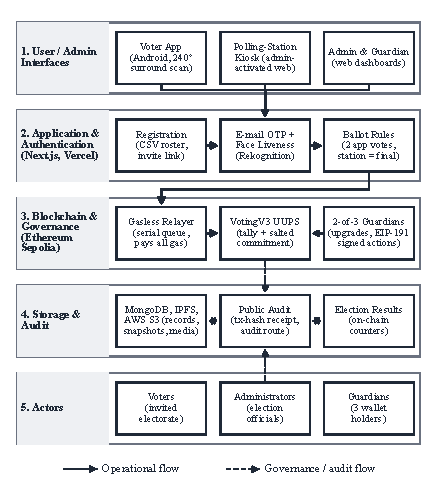
\includegraphics[width=\columnwidth]{fig_layers.pdf}
\caption{Layered view of BlockVote. Voters reach the chain only through the application tier and the gasless relayer; guardians govern contract upgrades, and anyone can check inclusion through the public audit route.}
\label{fig:layers}
\end{figure}

\begin{figure*}[t]
\centering
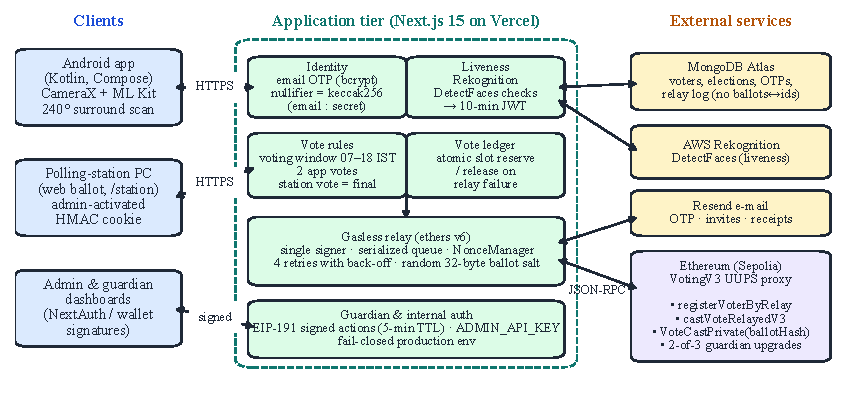
\includegraphics[width=\textwidth]{fig_architecture.pdf}
\caption{Architecture of the BlockVote hybrid decentralised e-voting system. Voters never hold keys: all chain writes are relayed by the application tier. Privileged operations require an administrator session, a guardian wallet signature, or an internal API key.}
\label{fig:arch}
\end{figure*}

\subsection{System Architecture and Authentication}
The voter starts from an invitation link (an HTTPS App Link that opens the Android app) and completes two authentication stages. The first confirms that the requester owns the invited e-mail account: a 6-digit OTP generated with \code{crypto.randomInt}, stored as a bcrypt hash, valid for 5\,min with at most 3 wrong attempts, and rate-limited to 5 requests per minute per IP, in line with NIST SP~800-63B guidance~\cite{nist80063b}. The second confirms that a live human is present at the device.

On Android, CameraX supplies the front-camera stream, analysed every 90\,ms by Google ML Kit, and \code{SensorManager} tracks device orientation. The voter rotates the phone in one direction until 240$^\circ$ of yaw are accumulated while keeping the face at 10--38\% of the frame height; any additional face resets the scan, and after 900\,ms of stable single-face framing the app auto-captures a frame. The server then calls AWS Rekognition \code{DetectFaces} and accepts the frame only if exactly one face is present with confidence $\geq 90$, brightness $\geq 30$, no eyeglasses or sunglasses detected with confidence $>80$, and eyes open. Success yields a 10-minute HS256 biometric JWT bound to the voter's nullifier.

This procedure makes simple presentation attacks, such as a photograph, paper cut-out or replayed video, more difficult; it is not proof that every presentation attack is stopped~\cite{iso30107}. The on-device motion test and the server-side image check are independent, so an attacker has to defeat both. Note that the server checks \emph{liveness and image quality}; it does not match the face against an enrolled reference.

\subsection{Voter Identity and Nullifiers}
The contract must recognise repeat participation without publishing an e-mail address. BlockVote derives a deterministic nullifier from the normalised e-mail and an off-chain server secret:
\begin{equation}
n = \mathrm{Keccak256}\big(\mathrm{clean}(\mathit{email})\,\|\,\text{``:''}\,\|\,K_{id}\big).
\label{eq:nullifier}
\end{equation}
The nullifier is a pseudonymous key in the per-election registration map \code{isRegisteredVoter[e][n]}, the vote-choice map \code{voteChoice[n][e]} and the revision counter \code{voteRevisionCount[n][e]}. The same voter has the same $n$ in every election; participation is separated because each map is indexed by the election identifier. An observer cannot recover the e-mail as long as $K_{id}$ stays secret, but this is a privacy-masking step, not an anonymous-credential scheme. In production, $K_{id}$ and all other secrets are read by a fail-closed configuration module that refuses to run when a value is missing.

\subsection{Gasless Relaying and Nonce Management}
In a wallet-based dApp the voter signs, broadcasts and pays for the transaction. BlockVote separates these duties: after the application checks succeed, the backend relay wallet calls the contract and pays the gas using ethers.js v6. A single relay account creates a nonce problem when requests arrive together. BlockVote therefore places relay requests in a promise queue, wraps the wallet in an ethers \code{NonceManager}, waits for each receipt before releasing the queue, and retries nonce errors up to four times with linear back-off. Every relayed call is an ordinary contract transaction logged with its gas usage, so the ledger still shows the complete sequence of submissions even though voters never touch a wallet. The queue also gives the operator one place to observe throughput and to pause submissions.

\subsection{Blinded Ballots and Bounded Re-Voting}
The contract function \code{castVoteRelayedV3}$(e,c,n,s)$ checks registration, the Voting phase and the candidate index, updates the tally, stores $c+1$ in \code{voteChoice}, and emits
\begin{equation}
\text{VoteCastPrivate}\big(e,\;\mathrm{Keccak256}(e\,\|\,c\,\|\,n\,\|\,s),\;\mathit{isRevote}\big),
\label{eq:ballot}
\end{equation}
where $s$ is a fresh 32-byte salt chosen by the relayer. The event contains neither the candidate nor the voter's plaintext identity; the random salt prevents testing candidate values against the event. If a previous choice exists and differs, the contract moves one unit from the old to the new candidate counter (with an underflow guard) and increments the revision counter, so the tally always reflects the latest choice. Unlike our earlier VotingV1, which emitted \code{VoteCast}$(e,c)$ and accepted exactly one ballot, V3 never publishes the candidate. The \emph{isRevote} flag gives observers an aggregate audit signal (revisions versus registered voters) without exposing any choice.

The contract itself permits unlimited revisions; the application tier bounds them (Fig.~\ref{fig:channels}). A remote voter may cast two app ballots, a first vote and one change, and a ballot cast at a polling station is final and overrides any app ballot. This helps a voter who was pressured at home: the coercer cannot obtain a reliable final receipt, and the voter can always cast a decisive vote in person, while limiting repeated pressure and relay cost. The policy is enforced by an atomic compare-and-increment on the voter document (Algorithm~\ref{alg:slot}), so concurrent requests cannot exceed the allowance. Ballots are also accepted only during configurable voting hours (default 07:00--18:00, Asia/Kolkata).

\begin{figure}[t]
\centering
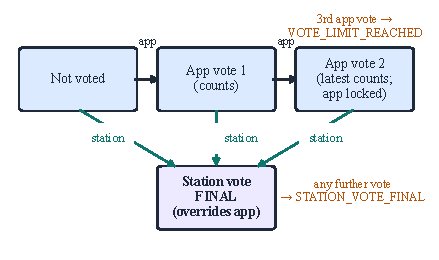
\includegraphics[width=\columnwidth]{fig_channels.pdf}
\caption{Per-voter ballot state machine across the app and polling-station channels.}
\label{fig:channels}
\end{figure}

\begin{algorithm}[t]
\caption{Atomic vote-slot reservation}
\label{alg:slot}
\footnotesize
\begin{algorithmic}[1]
\Require voter id $v$, channel $\in\{\text{app},\text{station}\}$, $M=2$
\State $F \gets \{\_id = v,\ \text{stationVoteFinal} \neq \text{true}\}$
\If{channel $=$ app} \State $F \gets F \wedge \neg(\text{votesCast} \geq M)$ \EndIf
\State $U \gets \{\text{votesCast} \mathrel{+}= 1\}$
\If{channel $=$ station} \State $U \gets U \cup \{\text{stationVoteFinal} \gets \text{true}\}$ \EndIf
\State $b \gets \textsc{FindOneAndUpdate}(F, U, \text{return before})$
\If{$b = \bot$} \Return reject (\textsc{Vote\_Limit\_Reached} or \textsc{Station\_Vote\_Final}) \EndIf
\State $r \gets \textsc{RelayCastVote}(\cdot)$
\If{$r$ failed} \State restore the voter document to $b$ (release slot) \EndIf
\end{algorithmic}
\end{algorithm}

Fig.~\ref{fig:seq} summarises the complete ballot flow. The voter's e-mail receipt contains the transaction hash but not the candidate, and a public audit route confirms inclusion of a transaction without revealing its content.

\begin{figure*}[t]
\centering
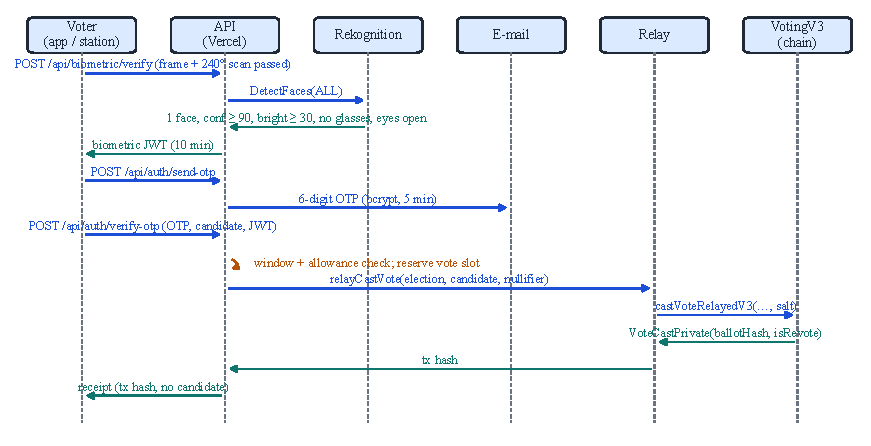
\includegraphics[width=0.94\textwidth]{fig_sequence.pdf}
\caption{Ballot-casting sequence. The candidate reaches the chain only inside contract storage; the public event carries a salted commitment.}
\label{fig:seq}
\end{figure*}

\subsection{Polling-Station Channel}
An authenticated administrator activates a computer for one election at \code{/station}. The server sets an \code{httpOnly}, \code{SameSite=Strict} cookie whose payload (station identifier and name, election, administrator, issue and expiry time; 16\,h lifetime) is authenticated with HMAC-SHA256. The web ballot at \code{/station/vote} renders only when this cookie verifies, so the web channel cannot be used remotely; the kiosk resets after 2 minutes of inactivity. Because the environment is supervised, the station ballot uses OTP and a face check but no surround scan.

\subsection{UUPS Governance and Guardian Authorisation}
VotingV3 uses the UUPS proxy model~\cite{eip1822}: the proxy holds election state while the implementation holds logic. An upgrade follows propose, approve and execute steps; execution requires an unexecuted proposal with at least two of three guardian approvals:
\begin{equation}
\mathit{UpgradeAccepted} =
\begin{cases}
1, & \text{approvalCount} \geq 2 \wedge \neg\text{executed},\\
0, & \text{otherwise.}
\end{cases}
\label{eq:upgrade}
\end{equation}
The threshold is checked on-chain at execution time, so the contract rather than an off-chain agreement enforces it. Two colluding guardians could still approve harmful code, and a careless storage-layout change could damage proxy state, so key custody, proposal review, and upgrade monitoring remain part of the deployment process. Privileged dashboard actions (approving an election go-live, wiping data, clearing relay history) require an EIP-191 signature~\cite{eip191} from a guardian wallet binding the action, target and issue time; the server recovers the signer, rejects signatures older than five minutes, and checks it against the configured and on-chain guardian lists. Server-to-server synchronisation routes require an API key compared in constant time.

\subsection{Security and Threat Model}
The attacker can inspect public blocks and events, make repeated requests, attempt multiple registrations, observe the voter interface, or compromise one administrative key. We do not assume that the phone, camera, biometric provider, e-mail provider, database, or relayer are automatically trustworthy, and we do not claim protection against a compromised blockchain majority or an attacker who controls the voter's device. The relay operator is trusted not to censor or alter ballots and learns the candidate at submission time. We consider adversaries A1 (ineligible or double voter), A2 (coercer), A3 (malicious administrator), A4 (compromised backend database), A5 (contract-logic attacks), A6 (relay and network attacks), and A8 (guardian collusion); each maps onto the adversarial test suite in Section~\ref{sec:results}. Table~\ref{tab:threat} summarises controls and remaining concerns.

\begin{table}[t]
\caption{Threat model and mitigations}
\label{tab:threat}
\centering
\footnotesize
\begin{tabular}{@{}p{1.45cm}p{3.35cm}p{2.95cm}@{}}
\toprule
\textbf{Threat} & \textbf{BlockVote control} & \textbf{Remaining concern} \\
\midrule
Duplicate voting & Per-election nullifier and vote-choice maps; later ballots replace rather than add; atomic slot ledger & Compromise of the identity service or $K_{id}$ \\
Sybil registration & Admin roll, OTP, liveness and image-quality checks before relay & No face-to-enrolment matching; false accepts/rejects untested at scale \\
Ballot observation & Salted commitment in event; receipts omit candidate & Relayer and backend see authenticated requests \\
Vote coercion & Two app ballots; final station override; voting-hours window & Coercion until polls close; device compromise \\
Nonce collision & Serialised queue, NonceManager, 4 retries & Relayer outage delays submissions \\
Malicious upgrade & 2-of-3 guardian UUPS gate & Two colluding guardians; no timelock \\
Forged admin action & EIP-191 guardian signatures (5\,min TTL); API key & Guardian key theft \\
\bottomrule
\end{tabular}
\end{table}

\subsection{Implementation}
The Android module hosts the Compose screens, Hilt dependency injection, repositories and the biometric scanning flow; it supports \code{blockvote://} deep links and verified HTTPS App Links, and its production flavour is restricted to HTTPS. The web workspace contains VotingV3, 56 Next.js API routes, 11 MongoDB models, the administrator dashboard (election setup, candidates, CSV roster upload), the guardian portal, the relay engine, identity utilities, storage integrations, and Hardhat configuration. Election phases (Registration, Voting, Completed) are managed inside the contract, which is the single source of truth. Off-chain services (MongoDB, IPFS, ImageKit) reduce on-chain data but need their own access control and retention policies. Tables~\ref{tab:stack} and~\ref{tab:loc} give the stack and code size.

\begin{table}[t]
\caption{Technology stack}
\label{tab:stack}
\centering
\footnotesize
\begin{tabular}{@{}ll@{}}
\toprule
\textbf{Layer} & \textbf{Technology (version)} \\
\midrule
Contract & Solidity 0.8.22, OpenZeppelin 5.6 (UUPS) \\
Chain & Hardhat 2.28 (local), Ethereum Sepolia (live) \\
Web / API & Next.js 15.3, React 19.1, Auth.js v5 \\
Chain client & ethers 6.15 (NonceManager relay) \\
Data / storage & MongoDB Atlas, Pinata IPFS, ImageKit \\
Biometrics & AWS Rekognition; ML Kit Face 16.1.7 \\
Android & Kotlin 2.2, Compose, Hilt 2.57, CameraX 1.5 \\
Hosting & Vercel (serverless functions) \\
\bottomrule
\end{tabular}
\end{table}

\begin{table}[t]
\caption{Code base metrics (source lines)}
\label{tab:loc}
\centering
\footnotesize
\begin{tabular}{@{}lrr@{}}
\toprule
\textbf{Component} & \textbf{Files} & \textbf{Lines} \\
\midrule
Solidity contracts (V1, V2, V3) & 3 & 959 \\
API route handlers & 56 & 4,735 \\
Web pages and components (JSX) & 44 & 7,699 \\
Server libraries (JS) & 37 & 2,865 \\
Android app (Kotlin) & 42 & 5,351 \\
\midrule
\textbf{Total} & \textbf{182} & \textbf{21,609} \\
\bottomrule
\end{tabular}
\end{table}

% =====================================================================
\section{Results and Discussions}
\label{sec:results}

\subsection{Evaluation Setup}
Two environments answer different questions. The in-process Hardhat network tests whether contract logic and the relay behave correctly without network propagation; Ethereum Sepolia tests behaviour when transactions must be broadcast and included in real blocks. Gas was measured with a reproducible script (\code{scripts/benchmark-gas.js}) that deploys the UUPS proxy and runs one election with 3 candidates and 50 voters, followed by 25 changed and 25 unchanged re-votes. The production relay log, containing 114 Sepolia transactions (12--21 August 2026) with receipt \code{gasUsed} and effective gas price, validates these numbers. Production latency was measured from a residential client in India with 20 sequential HTTPS requests per endpoint.

\subsection{Automated and End-to-End Testing}
All 190 automated tests pass (Table~\ref{tab:tests}). The adversarial suite covers the scenarios in Table~\ref{tab:attacks}. The production-readiness suite scans shipped source for development leftovers (test-network keys, hard-coded local URLs, demo toggles), verifies fail-closed configuration, and tests guardian signatures against forgery, expiry, cross-election replay, and non-guardian signers. The suites exposed two real defects that were fixed: 35 contract assertions still expected V1 revert strings, and a production endpoint failed on cold start because a referenced data model was not registered. A scripted end-to-end test against a running server confirmed seven rules: first app vote accepted; one change accepted; third app vote rejected; station vote accepted and overriding; app vote after station rejected; second station vote rejected; on-chain \code{getVoteStatus} consistent with the off-chain ledger. A station ballot in the browser and an app ballot on a physical Android phone were also completed with a live face.

\begin{table}[t]
\caption{Automated test suites (all passing)}
\label{tab:tests}
\centering
\footnotesize
\begin{tabular}{@{}lrl@{}}
\toprule
\textbf{Suite} & \textbf{Tests} & \textbf{Scope} \\
\midrule
VotingV3 contract & 75 & lifecycle, re-vote, tallies, UUPS \\
Security attacks (A1--A8) & 30 & adversarial scenarios \\
Production readiness & 26 & env, auth, links, source scan \\
Preflight \& identity & 22 & eligibility cache, commitments \\
Vote rules & 17 & hours, allowance, station token \\
Rate limiting & 13 & sliding window \\
Biometric tokens & 7 & landmarks, JWT \\
\midrule
\textbf{Total} & \textbf{190} & \\
\bottomrule
\end{tabular}
\end{table}

\begin{table}[t]
\caption{Adversarial scenarios in the security suite}
\label{tab:attacks}
\centering
\footnotesize
\begin{tabular}{@{}p{1.6cm}p{6.35cm}@{}}
\toprule
\textbf{Adversary} & \textbf{Representative tests} \\
\midrule
A1 Voter & unregistered vote; zero or null-byte nullifier; direct (non-relay) cast or registration; out-of-range candidate; salt replay \\
A2 Coercer & no plaintext candidate in events; legacy event not emitted; coerced vote overwritten; commitment brute-force resistance \\
A3 Admin & add candidate during voting; reopen completed election; single-guardian upgrade; direct counter write \\
A4 Backend & nullifier pre-image resistance; salt/identity correlation \\
A5 Contract & immutable config; underflow guard; phase machine; vote conservation \\
A6 Relay & revoked relay privileges; distinct salts yield distinct events \\
A8 Collusion & 2-of-3 guardians can upgrade; one cannot \\
\bottomrule
\end{tabular}
\end{table}

\subsection{Gas Consumption}
Table~\ref{tab:gas} and Fig.~\ref{fig:gas} report gas per operation. Registration and phase transitions match Sepolia exactly (55,697 and 38,619 gas), confirming the benchmark is representative; creation and candidate costs differ only because production strings differ in length. A first ballot costs 89,946 gas and a re-vote 77,478 (changed) or 63,974 (same candidate). Against the one-shot VotingV1 baseline (66,784 gas), commitments and re-vote bookkeeping add 23,162 gas (+34.7\%), dominated by one additional zero-to-non-zero storage write. These measurements supersede the 47,000--58,000 gas range reported for an earlier prototype.

\begin{table}[t]
\caption{Gas per operation (Hardhat: 50 voters; Sepolia: live relay log)}
\label{tab:gas}
\centering
\footnotesize
\begin{tabular}{@{}lrrr@{}}
\toprule
\textbf{Operation} & \textbf{V3 Hardhat} & \textbf{V3 Sepolia} & \textbf{V1 baseline} \\
 & mean (n) & mean (n) & mean \\
\midrule
Create election & 238,635 (1) & 223,253 (9) & 238,613 \\
Add candidate & 181,073 (3) & 193,002 (17) & 181,148 \\
Register voter & 55,697 (50) & 55,697 (83) & 55,752 \\
Phase transition & 38,619 (1) & 38,619 (5) & 38,585 \\
First vote & 89,946 (50) & -- & 66,784 \\
Re-vote, changed & 77,478 (25) & -- & n/a \\
Re-vote, same & 63,974 (25) & -- & n/a \\
\bottomrule
\end{tabular}
\end{table}

\begin{figure}[t]
\centering
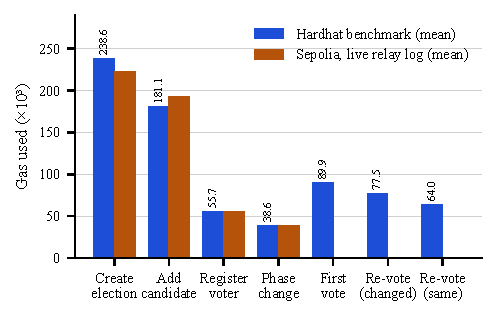
\includegraphics[width=\columnwidth]{fig_gas.pdf}
\caption{Gas per operation: benchmark vs.\ production (Sepolia) relay transactions.}
\label{fig:gas}
\end{figure}

\subsection{Operating Cost and Throughput}
Sponsoring ballots gives the operator a predictable cost per voter. With one ballot this is $G_1 = 55{,}697 + 89{,}946 = 145{,}643$ gas; the worst case (two app ballots and a station override) is $G_{\max} = 145{,}643 + 2\times 77{,}478 = 300{,}599$ gas. For $N$ voters at gas price $p$ gwei the cost is $C = N\,G\,p\cdot10^{-9}$~ETH. At the observed Sepolia median of 1.09~gwei one voter costs $1.59\times10^{-4}$~ETH; $10^4$ voters cost 1.46~ETH at 1~gwei and 29.1~ETH at 20~gwei (Fig.~\ref{fig:cost}). The 114 production transactions consumed 0.01224~ETH in total. Because the relayer waits for each receipt within one queue per server instance, throughput is bounded by roughly one confirmed transaction per block, about 300 ballots per hour at a 12\,s slot time, even though a 30\,M-gas block could hold 333 first ballots. Batching, pipelined nonces, or a layer-2 deployment would raise throughput and lower cost without contract changes.

\begin{figure}[t]
\centering
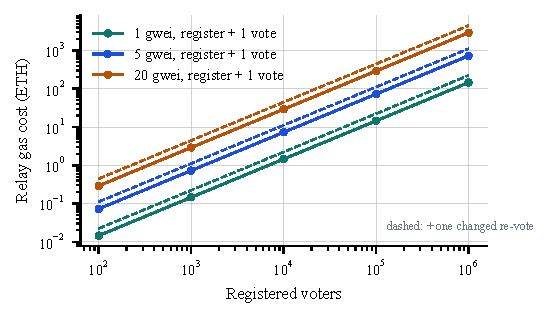
\includegraphics[width=\columnwidth]{fig_cost.pdf}
\caption{Projected relay cost versus electorate size for three gas prices.}
\label{fig:cost}
\end{figure}

\subsection{Latency}
Fig.~\ref{fig:latency} shows production round-trip latency: light endpoints have medians of 230--260\,ms and endpoints that query MongoDB and the chain 657--797\,ms; the p95 outliers (1.7\,s and 5.0\,s) are single samples consistent with serverless cold starts, and all 100 requests succeeded. The project evaluation log of an earlier prototype additionally reports the measurements in Table~\ref{tab:reported}; they were not re-run for this paper and are listed for completeness. The reported 12.4\,s mean Sepolia inclusion is consistent with Ethereum's 12\,s slot time and with the throughput bound above.

\begin{figure}[t]
\centering
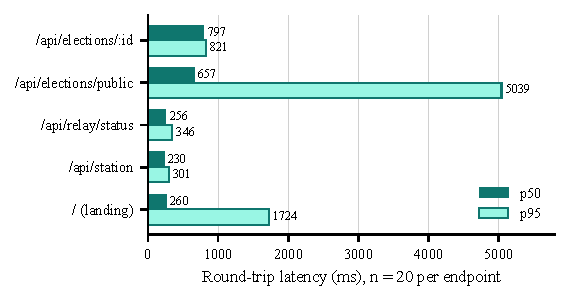
\includegraphics[width=\columnwidth]{fig_latency.pdf}
\caption{Production API latency (p50 and p95, 20 requests per endpoint).}
\label{fig:latency}
\end{figure}

\begin{table}[t]
\caption{Earlier prototype results reported in the project log}
\label{tab:reported}
\centering
\footnotesize
\begin{tabular}{@{}p{2.1cm}p{2.45cm}p{3.2cm}@{}}
\toprule
\textbf{Metric} & \textbf{Reported value} & \textbf{Interpretation} \\
\midrule
Local confirmation & 1.82\,s mean (0.34\,s S.D.) & Hardhat RPC responsiveness \\
Sepolia inclusion & 12.4\,s mean (2.8\,s S.D.) & Public testnet confirmation delay \\
Concurrent burst & 50 simultaneous requests, 100\% success & No nonce collisions in the test \\
Evaluation volume & 500 simulated ballots & Basis for latency observations \\
Static spoofing & 100\% rejection of tested 2D cases & Scenario-specific, not general PAD proof \\
\bottomrule
\end{tabular}
\end{table}

The reported 100\% rejection applies only to the static 2D spoofing cases used in the project test and must not be read as general presentation-attack resistance. A thorough biometric evaluation would report device classes, participant demographics, false-accept and false-reject rates, and a reproducible procedure~\cite{iso30107}.

\subsection{Comparison with Existing Systems}
Table~\ref{tab:compare} compares BlockVote with representative systems using properties reported in the cited literature. BlockVote's distinguishing combination is remote plus supervised channels with bounded re-voting (shared only with Estonian i-Voting), a public ledger without voter wallets or fees (unlike the Open Vote Network), and liveness-gated remote access. Its main weakness relative to Helios and the Open Vote Network is ballot secrecy against the operator: the relayer sees the plaintext choice, and \code{voteChoice} is readable by anyone who can compute nullifiers. All BlockVote transactions are issued by one relayer, so per-voter on-chain cost is hidden from the voter and independent of client capabilities.

\begin{table*}[t]
\caption{Qualitative comparison with existing voting systems (\cmark~provided, \pmark~partial or conditional, \xmark~not provided)}
\label{tab:compare}
\centering
\footnotesize
\resizebox{\textwidth}{!}{%
\begin{tabular}{@{}lcccccc@{}}
\toprule
\textbf{Property} & \textbf{EVM + VVPAT}~\cite{eci_evm} & \textbf{Estonia i-Voting}~\cite{madise2006,springall2014} & \textbf{Helios}~\cite{adida2008} & \textbf{Voatz}~\cite{specter2020} & \textbf{Open Vote Net.}~\cite{mccorry2017} & \textbf{BlockVote} \\
\midrule
Remote voting & \xmark & \cmark & \cmark & \cmark & \cmark & \cmark \\
Supervised in-person channel & \cmark & \cmark & \xmark & \xmark & \xmark & \cmark \\
Re-voting / in-person override & \xmark & \cmark & \pmark & \xmark & \xmark & \cmark~(bounded) \\
Public tamper-evident record & \xmark & \xmark & \cmark~(bulletin board) & \pmark~(permissioned) & \cmark & \cmark~(Ethereum) \\
Universally verifiable tally & \pmark~(paper audit) & \xmark & \cmark & \xmark & \cmark & \pmark~(on-chain counters) \\
Ballot secrecy vs.\ public & \cmark & \cmark & \cmark & \pmark & \cmark & \cmark~(commitments) \\
Ballot secrecy vs.\ operator & \cmark & \pmark~(key holders) & \pmark~(trustees) & \xmark & \cmark & \xmark~(relayer sees choice) \\
Automated liveness / biometrics & \xmark~(manual ID) & \xmark & \xmark & \cmark & \xmark & \cmark~(liveness only) \\
No voter wallet or fees & \cmark & \cmark & \cmark & \cmark & \xmark & \cmark \\
Upgrade governance & n/a & n/a & n/a & n/a & \xmark & \cmark~(2-of-3 UUPS) \\
Demonstrated scale & national & national & organisational & pilots & boardroom & prototype \\
\bottomrule
\end{tabular}}
\end{table*}

\subsection{Limitations}
The central trade-off is trust. Voters need no wallet or gas tokens, but the backend and relayer become critical services that can delay requests, observe authentication metadata, see each candidate choice, or become unavailable. The nullifier keeps e-mail addresses off the ledger but is linkable within and across elections and depends on the secrecy of $K_{id}$: a leak, together with the roster, would let an adversary reconstruct nullifiers and read \code{voteChoice}. Timing may let the backend associate an authentication event with a relay request, so the system should claim protection only against defined receipt-based coercion scenarios, not universal coercion resistance; bounded re-voting and the station override are operational, not cryptographic, defences~\cite{juels2005}.

Further gaps are: liveness without face-to-enrolment matching; go-live approval by one guardian (upgrades need two) and no upgrade timelock; per-instance in-memory rate limiting, which is weak on serverless platforms; per-instance relay throughput; minimal automated tests for the Android client; and a publicly readable gas-analytics endpoint. Formal verification of tally invariants, upgrade authorisation, event linkability and behaviour under dropped or reordered relay requests remains future work, as do client-side ballot encryption with threshold tallying, zero-knowledge biometric proofs, layer-2 deployment, and decentralised credentials that remove the dependence on institutional e-mail. These limitations are largely inherent to building on a public ledger; the value of the prototype is that it makes them explicit and testable.

% =====================================================================
\section{Conclusion}
BlockVote is a hybrid decentralised e-voting system that combines gasless relaying, salted Keccak-256 nullifiers, sensor-driven liveness, blinded ballot events, bounded multi-channel re-voting with a final polling-station override, and 2-of-3 UUPS upgrade governance. It removes voter-side gas payment and wallets, keeps plaintext identifiers and choices out of public events, lets a pressured voter correct a remote ballot and cast a decisive vote in person, and requires a guardian threshold for implementation upgrades. Measurements show 145,643 gas per voter (89,946 per first ballot), exact agreement between benchmark and Sepolia gas for shared operations, production API medians below 0.8\,s, and 190 passing automated tests including 30 adversarial scenarios. These results support the feasibility of the design for organisational elections such as student councils, corporate boards and cooperative societies, but do not establish readiness for public elections; independent contract review, biometric evaluation, privacy analysis, accessibility testing, and larger deployments remain necessary.

\section*{Artifact Availability}
The repository contains the gas benchmark (\code{Voting/scripts/benchmark-gas.js}), all test suites, and the measurement data and figure scripts used in this paper (\code{docs/paper/}).

\begin{thebibliography}{00}
\bibitem{saha2025} S. Saha, S. Barman, J. Dutta, S. Shaw and A. Sinha, ``A Secure and Transparent Blockchain driven E-Voting System using Smart Contract and IPFS-based Scalability,'' \emph{2025 IEEE Guwahati Subsection Conference (GCON)}, Itanagar, India, 2025, pp.~1--6, doi: 10.1109/GCON65540.2025.11173301.
\bibitem{nakamoto2008} S. Nakamoto, ``Bitcoin: A peer-to-peer electronic cash system,'' 2008. [Online]. Available: \url{https://bitcoin.org/bitcoin.pdf}
\bibitem{wood2014} G. Wood, ``Ethereum: A secure decentralised generalised transaction ledger,'' Ethereum Yellow Paper, 2014.
\bibitem{park2021} S. Park, M. Specter, N. Narula, and R. L. Rivest, ``Going from bad to worse: From Internet voting to blockchain voting,'' \emph{J. Cybersecurity}, vol.~7, no.~1, 2021.
\bibitem{abdulah2023} W. A. B. W. Abdulah and S. F. S. Adnan, ``Blockchain based Electronic Voting System Design with Smart Contracts,'' in \emph{Proc. 2023 IEEE Symp. on Computers \& Informatics (ISCI)}, 2023, doi: 10.1109/ISCI58771.2023.10391913.
\bibitem{gnanapriya2023} S. Gnanapriya, M. R. Eshwar, C. G. Shrikhiran, J. V. Chandar, and V. Nandhakumar, ``Secured Electronic voting system using Blockchain Technology,'' in \emph{Proc. 2023 Int. Conf. on Research Methodologies in Knowledge Management, Artificial Intelligence and Telecommunication Engineering (RMKMATE)}, 2023, doi: 10.1109/RMKMATE59243.2023.10369326.
\bibitem{singh2024} I. Singh, A. Kaur, P. Agarwal, and S. M. Idrees, ``Enhancing Security and Transparency in Online Voting through Blockchain Decentralization,'' \emph{SN Computer Science}, vol.~5, art. no.~921, 2024, doi: 10.1007/s42979-024-03286-2.
\bibitem{almadani2020} A. M. Al-madani, A. T. Gaikwad, V. Mahale, and Z. A. T. Ahmed, ``Decentralized e-voting system based on smart contract by using blockchain technology,'' in \emph{Proc. Int. Conf. Smart Innovations in Design, Environment, Management, Planning and Computing (ICSIDEMPC)}, 2020, pp.~176--180.
\bibitem{alvi2022} S. T. Alvi, M. N. Uddin, L. Islam, and S. Ahamed, ``DVTChain: A blockchain-based decentralized mechanism to ensure the security of digital voting system,'' \emph{J. King Saud Univ.--Comput. Inf. Sci.}, vol.~34, no.~9, pp.~6855--6871, 2022.
\bibitem{beydili2025} E. Beydili, U. C. Cabuk, G. Dalkilic, and Y. Ozturk, ``Securing Blockchain-based E-Voting through Shamir's Secret Sharing over Ethereum,'' 2025.
\bibitem{baniata2025} H. Baniata and G. E. Calu\~{n}a Chicaiza, ``BP-Vot: Blockchain-Based e-Voting Using Smart Contracts, Differential Privacy, and Self-Sovereign Identities,'' \emph{IEEE Access}, vol.~13, 2025, doi: 10.1109/ACCESS.2025.3548404.
\bibitem{panja2021} S. Panja \emph{et al.}, ``A secure end-to-end verifiable e-voting system using blockchain and cloud server,'' \emph{J. Inf. Secur. Appl.}, vol.~59, art.~102815, 2021, doi: 10.1016/j.jisa.2021.102815.
\bibitem{saim2022} M. Saim, M. Mamoon, I. Shah, and A. Samad, ``E-Voting via Upgradable Smart Contracts on Blockchain,'' in \emph{Proc. 2022 Int. Conf. on Futuristic Technologies (INCOFT)}, 2022, doi: 10.1109/INCOFT55651.2022.10094482.
\bibitem{eip1822} G. Barros and P. Gallagher, ``EIP-1822: Universal Upgradeable Proxy Standard (UUPS),'' Ethereum Improvement Proposals, 2019.
\bibitem{luo2021} T. Luo, ``An efficient blockchain based electronic voting system using proxy multi-signature,'' in \emph{Proc. 3rd Int. Academic Exchange Conf. Science and Technology Innovation (IAECST)}, 2021, pp.~513--516, doi: 10.1109/IAECST54258.2021.9695917.
\bibitem{chaum2004} D. Chaum, ``Secret-ballot receipts: True voter-verifiable elections,'' \emph{IEEE Security \& Privacy}, vol.~2, no.~1, pp.~38--47, 2004.
\bibitem{juels2005} A. Juels, D. Catalano, and M. Jakobsson, ``Coercion-resistant electronic elections,'' in \emph{Proc. ACM Workshop on Privacy in the Electronic Society (WPES)}, 2005, pp.~61--70.
\bibitem{eci_evm} Election Commission of India, ``Status paper on Electronic Voting Machine (EVM),'' New Delhi, India.
\bibitem{madise2006} \"U. Madise and T. Martens, ``E-voting in Estonia 2005: The first practice of country-wide binding Internet voting in the world,'' in \emph{Proc. Electronic Voting (EVOTE)}, GI LNI P-86, 2006, pp.~15--26.
\bibitem{springall2014} D. Springall \emph{et al.}, ``Security analysis of the Estonian Internet voting system,'' in \emph{Proc. ACM CCS}, 2014, pp.~703--715.
\bibitem{adida2008} B. Adida, ``Helios: Web-based open-audit voting,'' in \emph{Proc. 17th USENIX Security Symp.}, 2008, pp.~335--348.
\bibitem{benaloh2006} J. Benaloh, ``Simple verifiable elections,'' in \emph{Proc. USENIX/ACCURATE Electronic Voting Technology Workshop (EVT)}, 2006.
\bibitem{mccorry2017} P. McCorry, S. F. Shahandashti, and F. Hao, ``A smart contract for boardroom voting with maximum voter privacy,'' in \emph{Financial Cryptography and Data Security (FC)}, LNCS 10322, 2017, pp.~357--375.
\bibitem{specter2020} M. A. Specter, J. Koppel, and D. Weitzner, ``The ballot is busted before the blockchain: A security analysis of Voatz, the first Internet voting application used in U.S. federal elections,'' in \emph{Proc. 29th USENIX Security Symp.}, 2020, pp.~1535--1553.
\bibitem{somasekhar2024} G. Somasekhar, S. Jinka, C. K. Kanekal, and A. Marouthu, ``Digital Voting with Blockchain using Interplanetary File System and Practical Byzantine Fault Tolerance,'' \emph{Engineering, Technology \& Applied Science Research}, vol.~14, no.~6, pp.~19009--19015, 2024, doi: 10.48084/etasr.8440.
\bibitem{deepika2017} J. Deepika, S. Kalaiselvi, S. Mahalakshmi, and S. Agnes Shifani, ``Smart electronic voting system based on biometric identification---survey,'' in \emph{Proc. 3rd Int. Conf. Science Technology Engineering Management (ICONSTEM)}, 2017, pp.~939--942.
\bibitem{parmar2021} A. Parmar, S. Gada, T. Loke, Y. Jain, S. Pathak, and S. Patil, ``Secure e-voting system using blockchain technology and authentication via face recognition and mobile OTP,'' in \emph{Proc. 12th Int. Conf. Computing Communication and Networking Technologies (ICCCNT)}, Kharagpur, India, 2021, pp.~1--5, doi: 10.1109/ICCCNT51525.2021.9580147.
\bibitem{faruk2022} M. J. H. Faruk, M. Islam, F. Alam, H. Shahriar, and A. Rahman, ``Bie Vote: A biometric identification enabled blockchain-based secure and transparent voting framework,'' in \emph{Proc. 4th Int. Conf. Blockchain Computing and Applications (BCCA)}, 2022, pp.~253--258, doi: 10.1109/BCCA55292.2022.9922588.
\bibitem{sujatha2024} B. Sujatha, Y. Ganesh, N. Leelavathy, R. Tamilkodi, S. Venkatesh, B. Sandhya, and T. S. Kowshik, ``Blockchain-Powered E-Voting: A Novel Approach to Secure Voter Authentication, Online Voting and Election Automation,'' \emph{Indian Journal of Science and Technology}, vol.~17, no.~47, pp.~4948--4958, 2024, doi: 10.17485/IJST/v17i47.3573.
\bibitem{kalaiselvi2024} K. Kalaiselvi, K. Saravanan, S. M., T. Venkatesan, S. Ravi, and J. Karthi, ``Unleashing Innovation: Experimental Evaluation of Blockchain Assisted Electronic Voting System using Secured Authentication Scheme,'' in \emph{Proc. 2024 Int. Conf. on Intelligent Systems for Cybersecurity (ISCS)}, 2024, doi: 10.1109/ISCS61804.2024.10581204.
\bibitem{wu2018} H.-T. Wu and C.-Y. Yang, ``A blockchain-based network security mechanism for voting systems,'' in \emph{Proc. 1st Int. Cognitive Cities Conf. (IC3)}, 2018, pp.~227--230, doi: 10.1109/IC3.2018.00-15.
\bibitem{chavan2024} A. Chavan and A. Jadhav, ``Revolutionizing voting: Blockchain-powered e-voting with Solana,'' in \emph{Proc. 1st Int. Conf. Trends in Engineering Systems and Technologies (ICTEST)}, 2024. [Online]. Available: \url{https://ieeexplore.ieee.org/abstract/document/10576075}
\bibitem{hjalmarsson2018} F. P. Hj\'{a}lmarsson, G. K. Hrei\dh arsson, M. Hamdaqa, and G. Hj\'{a}lmt\'{y}sson, ``Blockchain-based e-voting system,'' in \emph{Proc. IEEE 11th Int. Conf. Cloud Computing (CLOUD)}, 2018, pp.~983--986.
\bibitem{kshetri2018} N. Kshetri and J. Voas, ``Blockchain-enabled e-voting,'' \emph{IEEE Software}, vol.~35, no.~4, pp.~95--99, 2018.
\bibitem{nist80063b} P. A. Grassi \emph{et al.}, ``Digital identity guidelines: Authentication and lifecycle management,'' NIST SP 800-63B, 2017.
\bibitem{iso30107} ISO/IEC 30107-3:2017, \emph{Information technology---Biometric presentation attack detection---Part 3: Testing and reporting}.
\bibitem{eip191} M. Swende and N. Johnson, ``EIP-191: Signed data standard,'' Ethereum Improvement Proposals, 2016.
\end{thebibliography}

\end{document}
